\chapter{Second Quantisation}

Before we begin our incursion into the so-called 'second quantisation', we need to appreciate the reason why the need for second quantization arose. The properties of quantum condensed matter systems and, by extension, that of real materials are controlled by the \textit{collective behaviour} of electrons in the presence of some background potential due to an underlying crystal lattice. This statement, in fact, is a simpler rendition of the Bohr-Oppenheimer approximation. So, what factors do we need to consider during the analysis of a condensed matter system?
\begin{itemize}
    \item Focus on electrons and their collective dynamics
    \item Electrons are free to move from one orbital to another (tunnelling/hopping)
    \item They are subject to a background potential from the lattice
    \item They can interact with each other due to Coulomb repulsion
\end{itemize}
The question remains, how do we formulate the Hamiltonian for many-body systems? How do we encode anti-symmetry of fermions into this many-particle wavefunction? And most importantly, how do we find out the eigenstates/eigenvalues of momentum and/or energy of the system?  \par

So, how do we encode fermionic anti-symmetry in many-particle wavefunctions? \par

Consider a single-particle quantum state $\phi_{\nu}(\vec{r})$, where $\nu$ refers to labels for the quantum state. The basis for a two-particle system is then given by 

\begin{equation*}
    \psi(\vec{r_{1}}, \vec{r_{2}}) = \frac{1}{\sqrt{2}}[\phi_{\nu_{1}}(\vec{r_{1}}) \phi_{\nu_{2}}(\vec{r_{2}}) - \phi_{\nu_{1}}(\vec{r_{2}}) \phi_{\nu_{2}}(\vec{r_{1}})]
\end{equation*}

This basis satisfies the anti-symmetry property, and also, there happens to be a less verbose manner through which we can express such wavefunctions - Slater's determinants. \par

For a generalized $N$-particle system such that the basis states are perfectly anti-symmetric under exchanging the labels of any two particles, the wavefunction can be expressed as

\begin{equation*}
    \psi(\vec{r_{1}}, \vec{r_{2}},..., \vec{r_{N}}) = \frac{1}{\sqrt{N!}} \begin{bmatrix}
        \phi_{\nu_{1}}(\vec{r_{1}}) & \phi_{\nu_{2}}(\vec{r_{1}}) & ... & \phi_{\nu_{N}}(\vec{r_{1}}) \\
        \phi_{\nu_{1}}(\vec{r_{2}}) & \phi_{\nu_{2}}(\vec{r_{2}}) & ... & \phi_{\nu_{N}}(\vec{r_{2}}) \\
        . & . &  & . \\
        . & . &  & . \\
        . & . &  & . \\
        \phi_{\nu_{1}}(\vec{r_{N}}) & \phi_{\nu_{2}}(\vec{r_{N}}) & ... & \phi_{\nu_{N}}(\vec{r_{N}})
    \end{bmatrix}
\end{equation*}

The 'first quantisation' principle cannot be used to satisfactorily explain condensed matter systems since calculations become cumbersome and expensive as the number of particles in the system increases, and the representation requires the number of particles, $N$, to be fixed. As $N$ approaches the limit associated with statistical physics, $N$ is allowed to fluctuate as per the grand canonical ensemble. Second quantisation or occupation number formalism is the standard way in which many-particle QM is formulated. It is based on the algebra of ladder operators.

\begin{itemize}
    \item Second quantisation provides a compact way of representing the many-body space of excitations.
    \item Properties of operators are now encoded in a single set of commutation/anti-commutation relations rather than in some explicit Hilbert space representation. 
\end{itemize}

In essence, second quantisation formalism offers us a significant computational advantage and a more compact and efficient representation of the Hamiltonian when dealing with many-particle quantum systems. For example, consider a \textit{symmetrised} $N$-particle wavefunction of fermions ($\zeta = -1$) or bosons ($\zeta = +1$) expressed in the form 

\begin{equation}
    \ket{\lambda_{1}, \lambda_{2},\ldots \lambda_{N}} = \frac{1}{\sqrt{N! \prod_{\lambda=0}^{\infty}n_{\lambda}!}} \sum_{\mathcal{P}}\zeta^{\mathcal{P}} \ket{\psi_{\lambda_{\mathcal{P}1}}} \otimes \ket{\psi_{\lambda_{\mathcal{P}2}}} \ldots \otimes \ket{\psi_{\lambda_{\mathcal{P}N}}}
\end{equation}

where $n_{\lambda}$ is the total number of particles in state $\lambda$ (for fermions, Pauli exclusion principle dictates that $n_{\lambda} = 0,1$, i.e. $n_{\lambda}! = 1$). The summation runs over all $N!$ permutations of the quantum numbers $\lambda_{i}$, and $\mathcal{P}$ denotes the parity \footnote{Parity is defined as the number of transpositions of two elements which brings the permutation ($\mathcal{P}_1, \mathcal{P}_2,\ldots \mathcal{P}_{N}$)) back to the ordered sequence (1,2,\ldots N)}. \par

Second quantisation formalism provides for a much more condensed and intuitive representation for the generalised wavefunction via the \textbf{vacuum state} $\ket{\Omega}$, and a set of creation (annihilation) \textbf{field operators} $c_{\lambda}$ ($c_{\lambda}^{\dagger}$), as follows:

\begin{equation}
\label{eq:eq1}
    c_{\lambda} \ket{\Omega} = 0, \quad \frac{1}{\sqrt{\prod_{\lambda}n_{\lambda}!}} c_{\lambda_N}^{\dagger} \ldots c_{\lambda_1}^{\dagger} \ket{\Omega} = \ket{\lambda_{1}, \lambda_{2},\ldots \lambda_{N}}
\end{equation}

In terms of physical interpretation, the operator $c_{\lambda}^{\dagger}$ creates a particle in state $\lambda$ while the operator $c_{\lambda}$ annihilates it. The commutation relations between these operators are captured via Clifford algebra \footnote{$[\hat{A},\hat{B}]_{\zeta} = \hat{A}\hat{B}-\zeta \hat{B}\hat{A}$ is the commutator $\zeta = 1$ (anticommutator $\zeta = -1$) for bosons (fermions). As per convention, the notation [.,.] denotes the commutator while \{.,.\} the anticommutator.}:

\begin{equation}
    [c_{\lambda},c_{\mu}^{\dagger}]_{-\zeta} = \delta_{\lambda,\mu}, \quad [c_{\lambda},c_{\mu}]_{-\zeta} = [c_{\lambda}^{\dagger},c_{\mu}^{\dagger}]_{-\zeta} = 0
\end{equation}

The physical interpretation of \ref{eq:eq1} and the commutation relations of the field operators is no trivial matter -- these equations imply that for \textit{any N}, the $N$-body wavefunction can be generated by an application of a set of $N$-independent operators to a vacuum state. Similarly, the formal definition of the general many-body or \textbf{Fock space} can be given as the direct sum $\oplus_{N=0}^{\infty}\mathcal{F}_N$, where $\mathcal{F}_N$ is defined as the linear span of all $N$-particle states $\ket{\lambda_{1}, \lambda_{2},\ldots \lambda_{N}} = \frac{1}{\sqrt{\prod_{\lambda}n_{\lambda}!}} c_{\lambda_N}^{\dagger} \ldots c_{\lambda_1}^{\dagger} \ket{\Omega}$. Intuitively, the Fock-subspaces $\mathcal{F}_N$ are generated by repeated action of creation operators on the vacuum space $\mathcal{F}_0$, and application of creation/annihilation field operator on a wavefunction takes it from one Fock-subspace to another. \par 

Before proceeding further, we need to determine the basis transformation for the field operators, and the Fourier transform of the operators from the real space to $k$-space (otherwise known as the momentum space). These results will prove incredibly useful while analysing the Hamiltonians for interacting fermionic systems. \par

\clearpage

\subsection{Change of basis}

The identity operator, $\mathcal{I}$ can be resolved as $\mathcal{I} = \sum_{\lambda=0}^{\infty}\ket{\lambda}\bra{\lambda}$. Using the relations $\ket{\tilde{\lambda}} = \sum_{\lambda}\ket{\lambda}\braket{\lambda|\tilde{\lambda}}$, $\ket{\lambda} = a_{\lambda}^{\dagger}\ket{\Omega}$, and $\ket{\tilde{\lambda}} = a_{\tilde{\lambda}}^{\dagger} \ket{\Omega}$, the transformation law is given by:

\begin{equation}
    c_{\tilde{\lambda}}^{\dagger} = \sum_{\lambda} \langle \lambda|\tilde{\lambda} \rangle c_{\lambda}^{\dagger}, \quad c_{\tilde{\lambda}} = \sum_{\lambda} \langle \tilde{\lambda}|\lambda \rangle c_{\lambda}
\end{equation}

\subsection{Fourier transform of field operators}

The physical interpretation provided for the creation (annihilation) operators states that they can be thought of as creating (annihilating) a particle in a state $\lambda$. In particular, this can be thought of as creating (annihilating) a particle at a dimensional site $r$, or equivalently, with a momentum $k$. This distinction is important since it is subtly related to the Heisenberg Uncertainty Principle -- the first scenario implies that the position of the particle is known with a very high certainty, and therefore is delocalised in momentum space and vice-versa. The transformation from real space to $k$-space and vice-versa is captured via Fourier transform of the field operators.

\begin{equation}
    \hat{c}_{r}^{(\dagger)} = \frac{1}{\sqrt{N}}\sum_{k}e^{-(+)ikr} \hat{c}_{k}^{(\dagger)}, \quad \hat{c}_{k}^{(\dagger)} = \frac{1}{\sqrt{N}}\int_{r}e^{-(+)ikr} \hat{c}_{r}^{(\dagger)}
\end{equation}

If we are dealing with discrete lattice sites, the Fourier transform has to be modified accordingly

\begin{equation}
    \hat{c}_{r}^{(\dagger)} = \frac{1}{\sqrt{N}} \sum_{k}e^{-(+)ikar}c_{k}^{(\dagger)}
\end{equation}

and $k$ lies inside the first Brillouin zone, i.e. $k \in \left[-\frac{\pi}{a},\frac{\pi}{a}\right]$ and $a$ is the lattice constant.

\section{Representation of operators}

Single particle or one-body operators $\hat{\mathcal{O}_{1}}$ acting in a $N$-particle Hilbert space, $\mathcal{F}^{N}$, generally take the form $\hat{\mathcal{O}_{1}} = \sum_{n = 1}^{N}\hat{o}_{n}$, where $\hat{o}_{n}$ is an ordinary single-particle operator acting on the $n$-th particle. A typical example is the kinetic energy operator $\hat{T} = \sum_{n}\frac{\hat{p}_{n}^{2}}{2m}$, where $\hat{p}_{n}$ is the momentum operator acting on the $n$-th particle. Since we have seen that, by applying field operators to the vacuum space, we can generate the Fock space in general and any $N$-particle Hilbert space in particular, it must be possible to represent any operator $\hat{\mathcal{O}_{1}}$ using the set of creation/annihilation operators. Here, we present the formal representation of a one-body operator using second quantization principles,

\begin{equation}
    \hat{\mathcal{O}_{1}} = \sum_{\lambda \mu \nu}\langle \mu | \lambda \rangle o_{\lambda}\langle \lambda | \nu \rangle \hat{c}^{\dagger}_{\mu} \hat{c}_{\nu} = \sum_{\mu \nu}\langle \mu|\hat{o}|\nu \rangle \hat{c}^{\dagger}_{\mu} \hat{c}_{\nu}
\end{equation}

Formally, the one-body operator, $\hat{\mathcal{O}_{1}}$, scatters a particle from a state $\nu$ into a state $\mu$ with probability amplitude $\braket{\mu|\hat{o}|\nu}$. \\

Two-body operators $\hat{\mathcal{O}_{2}}$ are needed to describe \textit{pairwise interactions} between particles. Although pair-interaction potentials are straightforwardly included in classical many-body theories, their embedding into conventional many-body quantum mechanics is made awkward by particle indistinguishability. Here again, we present the formal representation of a two-body operator using second quantization principles without providing a detailed derivation for the same.

\begin{equation}
    \hat{\mathcal{O}_{2}} = \sum_{\lambda \lambda^{\prime} \mu \mu^{\prime}} \langle \mu, \mu^{\prime}|\mathcal{O}_{2}|\lambda, \lambda^{\prime}\rangle \hat{c}_{\mu^{\prime}}^{\dagger} \hat{c}_{\mu}^{\dagger} \hat{c}_{\lambda} \hat{c}_{\lambda^{\prime}}
\end{equation}


\section{Tight Binding Models}

The beautiful simplicity embodied within the second quantisation formalism culminates with the ease with which it can be used to describe a many-particle system. Consider, for example, the free electron gas, with electrons occupying quantum states $\ket{k} = \ket{n_{k}}$, whose Hamiltonian can be expressed as

\begin{equation}
    \hat{H} = \sum_{k}\epsilon_{k}\hat{c}_{k}^{\dagger}\hat{c}_{k} = \sum_{k}\epsilon_{k}\hat{n}_{k}
\end{equation}

where $\epsilon_{k}$ represents the single-particle state of energy corresponding to the potential energy associated with orbital $\ket{k}$, and $\hat{n}_{k}$ represents the number operator. \par

Now, we shall introduce an additional layer of complexity to the problem by accounting for the interaction between fermionic particles constituting the system.

\begin{equation}
    \hat{H} = \sum_{i}\epsilon_{i} \: \hat{c}_{i}^{\dagger} \hat{c}_{i} + \sum_{i \neq j}t_{ij} \: \hat{c}_{i}^{\dagger} \hat{c}_{j}
\end{equation}

where $t_{ij}$ is the tunnelling matrix element corresponding to the tunnelling/hopping of an electron from orbital $\ket{i}$ to orbital $\ket{j}$, such that $\langle i|\hat{H}|j \rangle = t_{ij}$. Additionally, since the Hamiltonian is intrinsically Hermitian, it places a restriction on the elements of the tunnelling matrix, namely, $t_{ij} = t_{ji}^{*}$. Such tight-binding models can be used as a compact, and highly intuitive description of many-particle systems in terms of creation (annihilation) field operators. \par

Benzene provides an excellent toy model to illustrate the application of these principles to formulate its equivalent tight-binding Hamiltonian. The $p_{z}$ orbitals in benzene interact with only their nearest neighbors, which greatly simplifies the hopping terms associated with its $\pi$-bonded electronic network. 

\begin{equation*}
    \hat{H}_{\pi} = \epsilon \sum_{i=1}^{6} \hat{c}_{i}^{\dagger} \hat{c}_{i} + t \sum_{i=1}^{6} (\hat{c}_{i}^{\dagger} \hat{c}_{i+1} + \hat{c}_{i+1}^{\dagger} \hat{c}_{i})
\end{equation*}

\vspace{1cm}

\begin{figure}[h]
\centering
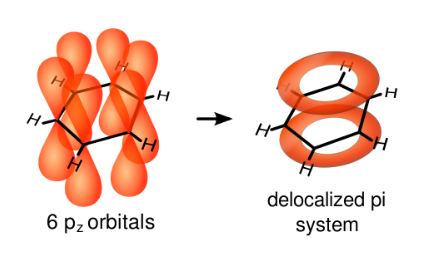
\includegraphics[scale=0.7]{benzene.png}
\caption{\textit{The $p_{z}$ orbitals of the respective carbon atoms in benzene interact with their nearest neighbours, forming a delocalized network of $\pi$-electrons}}\label{benzene}
\end{figure}